\documentclass[10pt]{article}
\usepackage[T1]{fontenc}
\usepackage{lmodern,amsmath,amssymb,booktabs,array,graphicx,tikz,pgfplots}
\usepackage[paperwidth=190mm,paperheight=224mm,margin=10mm]{geometry}
\usepackage[hidelinks]{hyperref}
\hypersetup{pdfauthor={},pdftitle={Monochrome mathematical illustrations: semiconductor-health identifiability}}
\usetikzlibrary{arrows.meta,positioning,calc,patterns}
\pgfplotsset{compat=1.18}
\newcommand{\trans}{^{\mathsf T}}\newcommand{\R}{\mathbb R}
\newcommand{\one}{\mathbf 1}\newcommand{\zero}{\mathbf 0}
\DeclareMathOperator{\rank}{rank}\DeclareMathOperator{\range}{range}
\DeclareMathOperator{\diag}{diag}\DeclareMathOperator{\Cov}{Cov}
\DeclareMathOperator{\Var}{Var}\DeclareMathOperator{\spanop}{span}
\newcommand{\FigureNote}{Visualization code prepared with assistance from OpenAI Codex.}
\pagestyle{empty}\setlength{\parindent}{0pt}
\tikzset{
 every picture/.style={font=\fontsize{9}{11}\selectfont,>=Latex},
 every node/.style={font=\fontsize{9}{11}\selectfont,inner sep=2pt},
 head/.style={font=\fontsize{9.5}{12}\selectfont\bfseries,anchor=west},
 tinytext/.style={font=\fontsize{8}{10}\selectfont},eq/.style={align=center},
 wire/.style={draw=black,line width=.5pt},arr/.style={->,black,line width=.65pt},
 device/.style={draw,fill=white,minimum width=1.1cm,minimum height=.38cm}}
\pgfplotsset{mathaxis/.style={axis lines=left,axis line style={black,line width=.5pt},
 tick style={black},tick label style={font=\fontsize{8}{10}\selectfont},
 label style={font=\fontsize{8.5}{10}\selectfont},grid=major,
 major grid style={black!15,line width=.2pt},
 legend style={font=\fontsize{8}{10}\selectfont,draw=none,fill=white},
 every axis plot/.append style={black}}}
\newcommand{\PlateTitle}[2]{\small\textbf{Mathematical plate #1}\hfill Monochrome TikZ / PGFPlots\par
 \vspace{1.5mm}{\large\bfseries #2}\par\vspace{2mm}}
\newcommand{\PlateCaption}[1]{\par\vspace{1mm}{\fontsize{8.5}{10.5}\selectfont #1\par
 \vspace{1mm}\FigureNote\par}}

\begin{document}
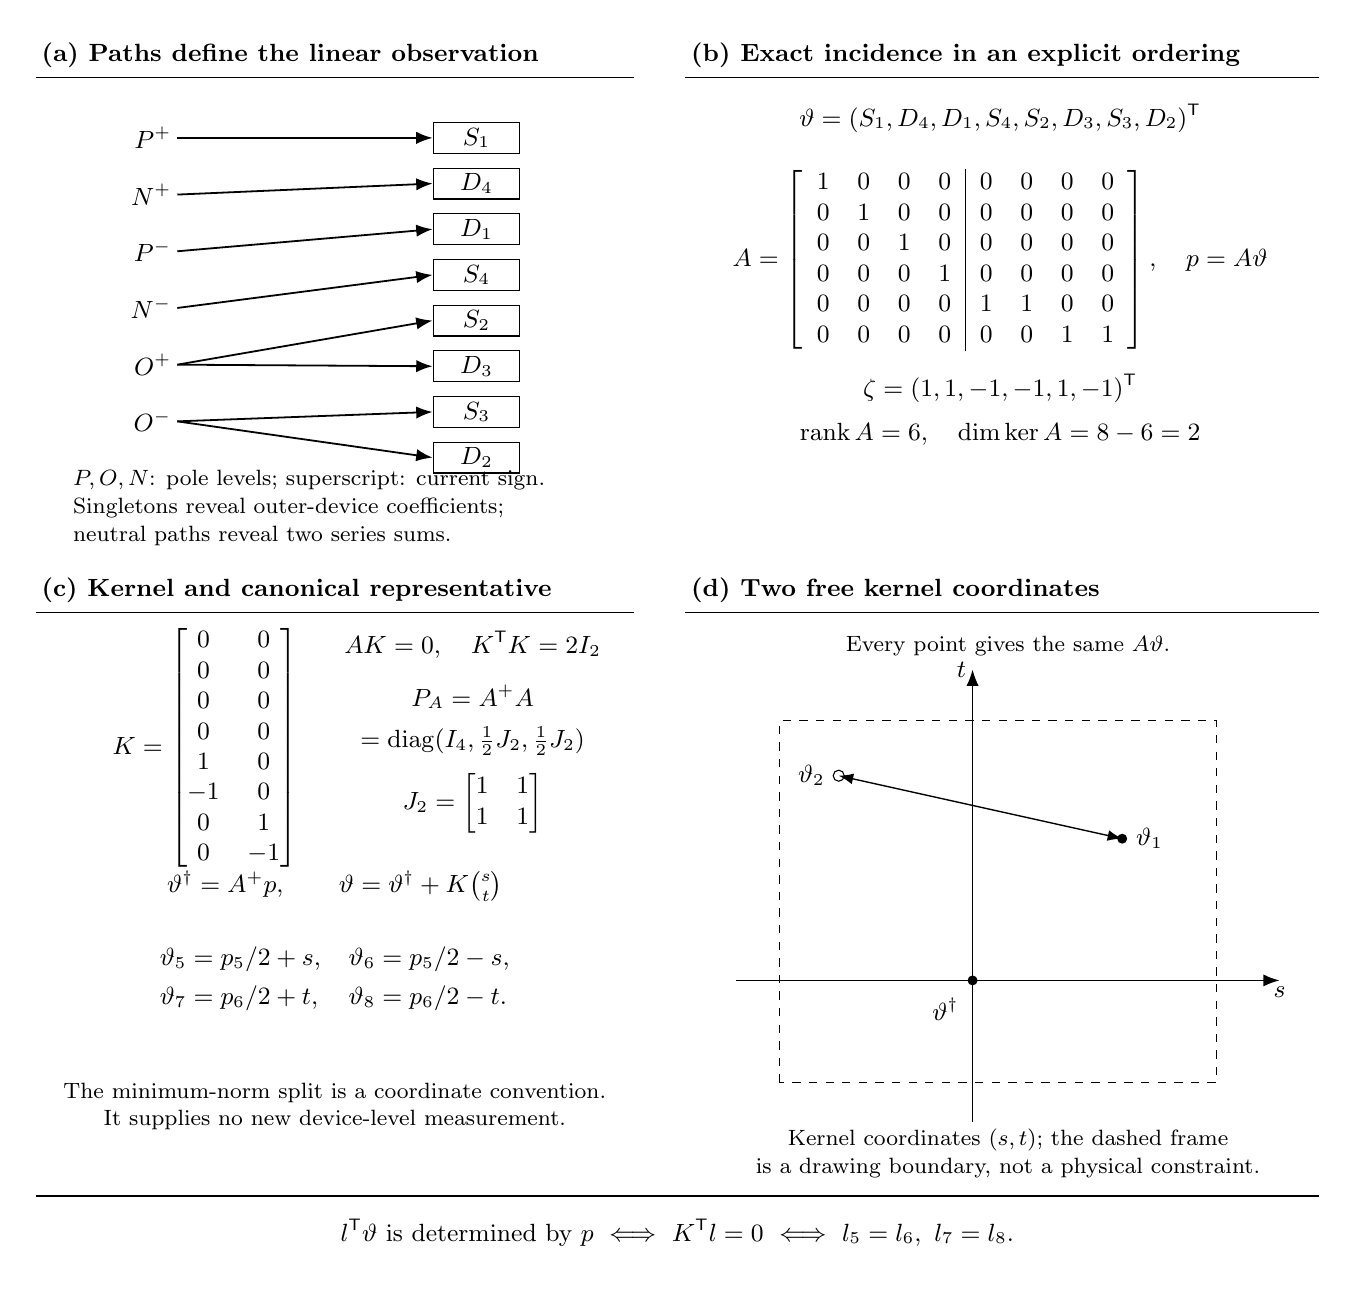
\begin{tikzpicture}[x=1cm,y=1cm]\path[use as bounding box] (0,0) rectangle (16.6,15.8);
\node[head] at (0.1,15.45){(a) Paths define the linear observation};\draw[wire] (0.1,15.17)--(7.699999999999999,15.17);
\node[head] at (8.35,15.45){(b) Exact incidence in an explicit ordering};\draw[wire] (8.35,15.17)--(16.4,15.17);
\node[anchor=east] (p0) at (1.9,14.4){$P^+$};
\node[anchor=east] (p1) at (1.9,13.68){$N^+$};
\node[anchor=east] (p2) at (1.9,12.96){$P^-$};
\node[anchor=east] (p3) at (1.9,12.24){$N^-$};
\node[anchor=east] (p4) at (1.9,11.52){$O^+$};
\node[anchor=east] (p5) at (1.9,10.8){$O^-$};
\node[device] (d0) at (5.7,14.4){$S_1$};
\node[device] (d1) at (5.7,13.82){$D_4$};
\node[device] (d2) at (5.7,13.24){$D_1$};
\node[device] (d3) at (5.7,12.66){$S_4$};
\node[device] (d4) at (5.7,12.08){$S_2$};
\node[device] (d5) at (5.7,11.5){$D_3$};
\node[device] (d6) at (5.7,10.920000000000002){$S_3$};
\node[device] (d7) at (5.7,10.34){$D_2$};
\draw[arr] (p0.east)--(d0.west);
\draw[arr] (p1.east)--(d1.west);
\draw[arr] (p2.east)--(d2.west);
\draw[arr] (p3.east)--(d3.west);
\draw[arr] (p4.east)--(d4.west);
\draw[arr] (p4.east)--(d5.west);
\draw[arr] (p5.east)--(d6.west);
\draw[arr] (p5.east)--(d7.west);
\node[tinytext,align=left,anchor=west] at (.5,9.7){$P,O,N$: pole levels; superscript: current sign.\\
Singletons reveal outer-device coefficients;\\neutral paths reveal two series sums.};
\node[eq] at (12.35,14.65){$\vartheta=(S_1,D_4,D_1,S_4,S_2,D_3,S_3,D_2)\trans$};
\node[eq] at (12.35,12.85){$A=\left[\begin{array}{cccc|cccc}
1&0&0&0&0&0&0&0\\0&1&0&0&0&0&0&0\\0&0&1&0&0&0&0&0\\0&0&0&1&0&0&0&0\\
0&0&0&0&1&1&0&0\\0&0&0&0&0&0&1&1
\end{array}\right],\quad p=A\vartheta$};
\node[eq] at (12.35,10.95){$\zeta=(1,1,-1,-1,1,-1)\trans$\\[5pt]
$\rank A=6,\quad\dim\ker A=8-6=2$};
\node[head] at (0.1,8.65){(c) Kernel and canonical representative};\draw[wire] (0.1,8.370000000000001)--(7.699999999999999,8.370000000000001);
\node[head] at (8.35,8.65){(d) Two free kernel coordinates};\draw[wire] (8.35,8.370000000000001)--(16.4,8.370000000000001);
\node[eq] at (2.25,6.65){$K=\begin{bmatrix}
0&0\\0&0\\0&0\\0&0\\1&0\\-1&0\\0&1\\0&-1\end{bmatrix}$};
\node[eq] at (5.65,6.85){$AK=0,\quad K\trans K=2I_2$\\[8pt]
$P_A=A^+A$\\[4pt]$=\diag(I_4,\tfrac12J_2,\tfrac12J_2)$\\[5pt]
$J_2=\begin{bmatrix}1&1\\1&1\end{bmatrix}$};
\node[eq] at (3.9,4.9){$\vartheta^\dagger=A^+p,\qquad\vartheta=\vartheta^\dagger+K\binom{s}{t}$};
\node[eq] at (3.9,3.72){$\begin{aligned}
\vartheta_5&=p_5/2+s,&\vartheta_6&=p_5/2-s,\\
\vartheta_7&=p_6/2+t,&\vartheta_8&=p_6/2-t.\end{aligned}$};
\node[tinytext,align=center] at (3.9,2.1){The minimum-norm split is a coordinate convention.\\It supplies no new device-level measurement.};
\draw[arr] (9.0,3.7)--(15.9,3.7) node[below] {$s$};
\draw[arr] (12.0,1.9)--(12.0,7.65) node[left] {$t$};
\draw[dashed,wire] (9.55,2.4) rectangle (15.1,7.0);
\fill (12,3.7) circle(1.8pt);\node[anchor=north east] at (11.9,3.55){$\vartheta^\dagger$};
\fill (13.9,5.5) circle(1.8pt);\node[anchor=west] at (14.0,5.5){$\vartheta_1$};
\draw[fill=white] (10.3,6.3) circle(2pt);\node[anchor=east] at (10.2,6.3){$\vartheta_2$};
\draw[<->,wire] (10.3,6.3)--(13.9,5.5);
\node[tinytext,align=center] at (12.45,7.95){Every point gives the same $A\vartheta$.};
\node[tinytext,align=center] at (12.45,1.5){Kernel coordinates $(s,t)$; the dashed frame\\is a drawing boundary, not a physical constraint.};
\draw[wire] (.1,.96)--(16.4,.96);
\node[eq] at (8.25,.5){$l\trans\vartheta\text{ is determined by }p\ \Longleftrightarrow\ K\trans l=0
\ \Longleftrightarrow\ l_5=l_6,\ l_7=l_8.$};\end{tikzpicture}
\end{document}
